\section{Versuchsanordnung und -durchführung}

\subsection{Versuchsaufbau}

Der Aufbau dieses Versuchs ist in Abbildung \ref{Aufbau} schematisch dargestellt und besteht aus einer Vakuumkammer, zwei Detektoren, drei Mylar-Folien, einer Strahlungsquelle, der signalverarbeitenden Elektronik sowie einem Computer.
\begin{figure}[H]
	\centering
	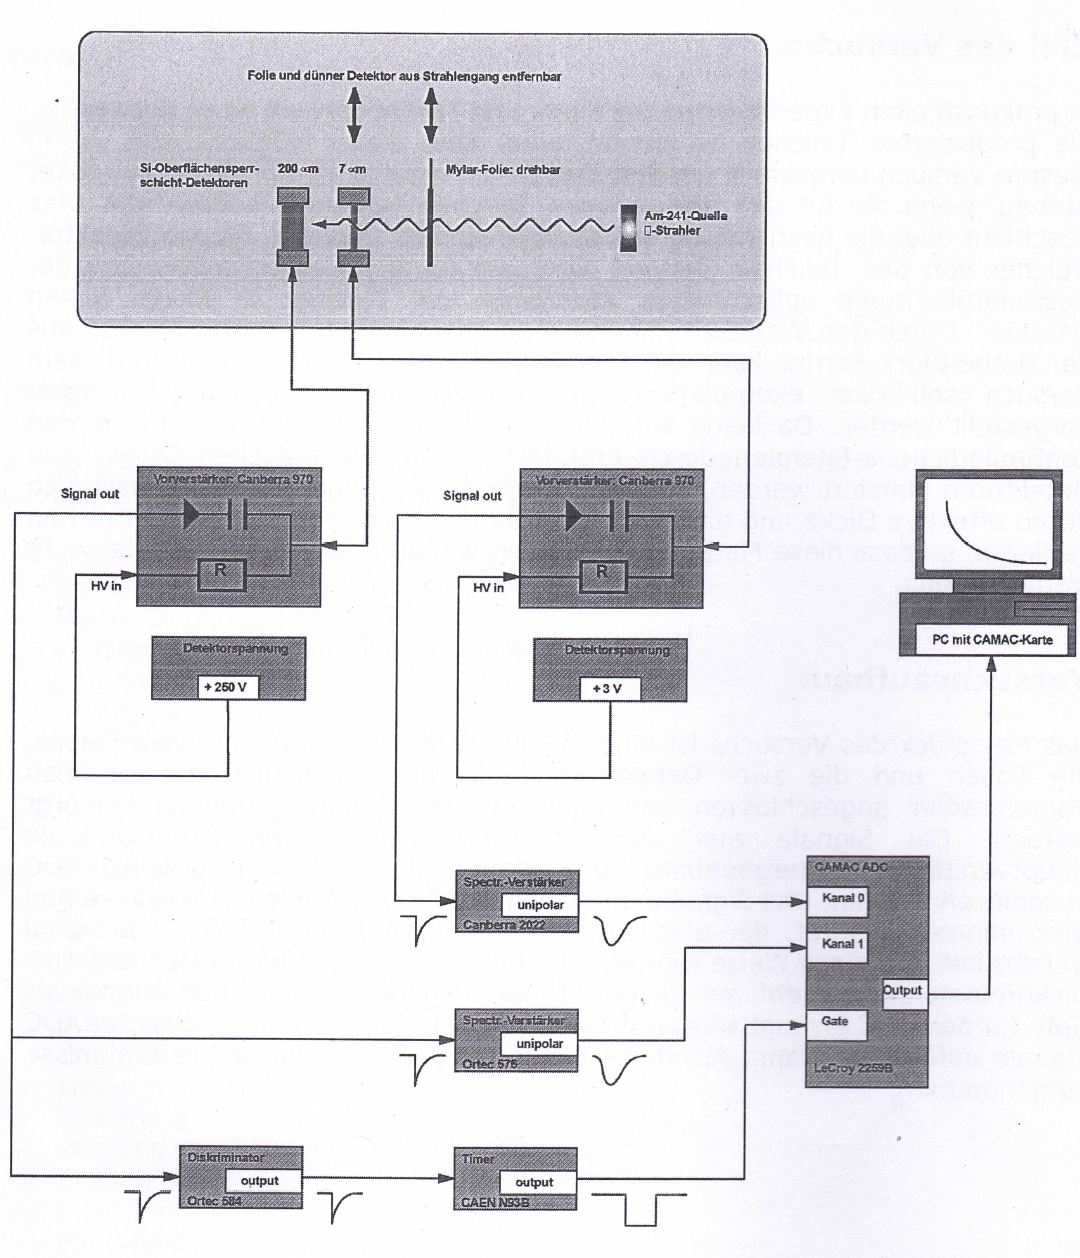
\includegraphics[width=1.0\textwidth]{img/Aufbau}
	\caption{In dieser Abbildung ist der schematische Aufbau dieses Versuchs in Form eines Blockschaltbilds dargestellt. Die Abbildung wurde der Versuchsanleitung\cite{wwu} entnommen und anschließend bearbeitet.}
	\label{Aufbau}
\end{figure}
\noindent Die Strahlungsquelle ist Americium-$241$, welches nahezu ausschließlich unter Emission von $\alpha$-Strahlung in angeregte Kernzustände von Neptunium-$237$ zerfällt.
Im Innern der Vakuumkammer ist die Strahlungsquelle auf einen Folienhalter gerichtet, in welchem drei unterschiedlich dicke Mylar-Folien eingesetzt sind.
Durch die Drehung der Folien lässt sich deren effektive Dicke verändern, sodass die Energie der hindurchgehenden $\alpha$-Teilchen variiert wird und kontinuierliche $\alpha$-Energien entstehen.
Hinter dem Folienhalter sind nacheinander die zwei Detektoren positioniert.
Bei den beiden Detektoren handelt es sich um mit Hochspannung (Abkürzung: HV) betriebene Halbleiterdetektoren, genauer gesagt Si-Oberflächensperrschicht-Detektoren.
Dabei ist der von einem einfallenden $\alpha$-Teilchen zuerst getroffene Detektor ungefähr $7\,$cm dick und wird als $\Delta E$-Detektor bezeichnet.
Der dem $\Delta E$-Detektor nachstehende sogenannte $E$-Detektor ist circa $20\,$cm dick.
An den $\Delta E$-Detektor wird eine Spannung von $+3\,$V und an den $E$-Detektor eine Spannung von $+250\,$V angelegt.
Die Folien und der $\Delta E$-Detektor sind aus dem Strahlengang entfernbar.
Beide Detektoren sind jeweils an Vorverstärker mit der Modellbezeichnung \glqq Canberra 970\grqq\ angeschlossen, welche über externe Spannungsquellen versorgt werden.


%Computer mit ADC und CAMAC-Karte.
%Diese ist über einen ADC (engl. \emph{analog-to-digital converter}) mit dem Computer verbunden, welcher über eine entsprechende Datenaufnahme-Software verfügt und somit den Zähler bildet.

\subsection{Elektronik}



\subsection{Durchführung}


